\documentclass[10pt]{beamer}
\usetheme{Rochester}
\usepackage[utf8]{inputenc}
\usepackage{amsmath}
\usepackage{amsfonts}
\usepackage{amssymb}
\usepackage[export]{adjustbox}
\setbeamertemplate{footline}[frame number]
\author{Justin Anguiano}
\title{Performance Optimization}
%\setbeamercovered{transparent} 
%\setbeamertemplate{navigation symbols}{} 
%\logo{} 
%\institute{} 
%\date{} 
%\subject{} 
\begin{document}

\begin{frame}
\titlepage
\end{frame}

%\begin{frame}
%\tableofcontents
%\end{frame}

\begin{frame}{}
Goal --- Improve Physics analysis performance \\
\quad \quad \\
Use different C/Python approaches to obtain a low programming overhead but high performance\\ 
\end{frame}

\begin{frame}
\textbf{Task to be optimized: Read File(s) containing a TTree, produce histograms from elements of the tree(s), write histograms to a TFile}\\
\quad \quad \\
\scriptsize
\textbf{ Three histograms are produced: TH1D: track $p_{T}$ weighted by $1/p_{T}$, TH1D: track $p_z$, TH2D, track $p_x$ vs $p_y$} \\
\normalsize
\quad \quad \\
First attempt using ROOT6 parallelization on local machine (laptop)\\
methods:\\
\begin{itemize}
\item Sequential run over a test file with TTreeReader (Compiled and Interpreted)
\item Parallelized run over a test file with TTreeReader (Compiled and Interpreted)
\end{itemize}

Test File Details\\
\begin{itemize}
\item code adapted from example: \url{https://root.cern.ch/doc/v612/imt101__parTreeProcessing_8C.html} 
\item uses fake event file containing 48000 events; each with some number of tracks per event
\item total tracks overall $\approx 2.4e+7$ 
\end{itemize}

\end{frame}


\begin{frame}
First Test Results:\\
\begin{columns}
	\begin{column}{0.5\textwidth}
	\begin{itemize}
		\scriptsize
		\item Time is Mean time $\pm$ stdev over 10 trials
		\item no guarantee of system releasing requested resources (nthreads) so perform multiple trials
		\item data point at nThreads = 0 is the basic sequential program
		\item high threadcount performance possibly bottlenecked by system?
		\item Takeaway: Compiling is important! $\approx $Factor of 2 improvement
	\end{itemize}
	\end{column}
	\begin{column}{0.5\textwidth}
   		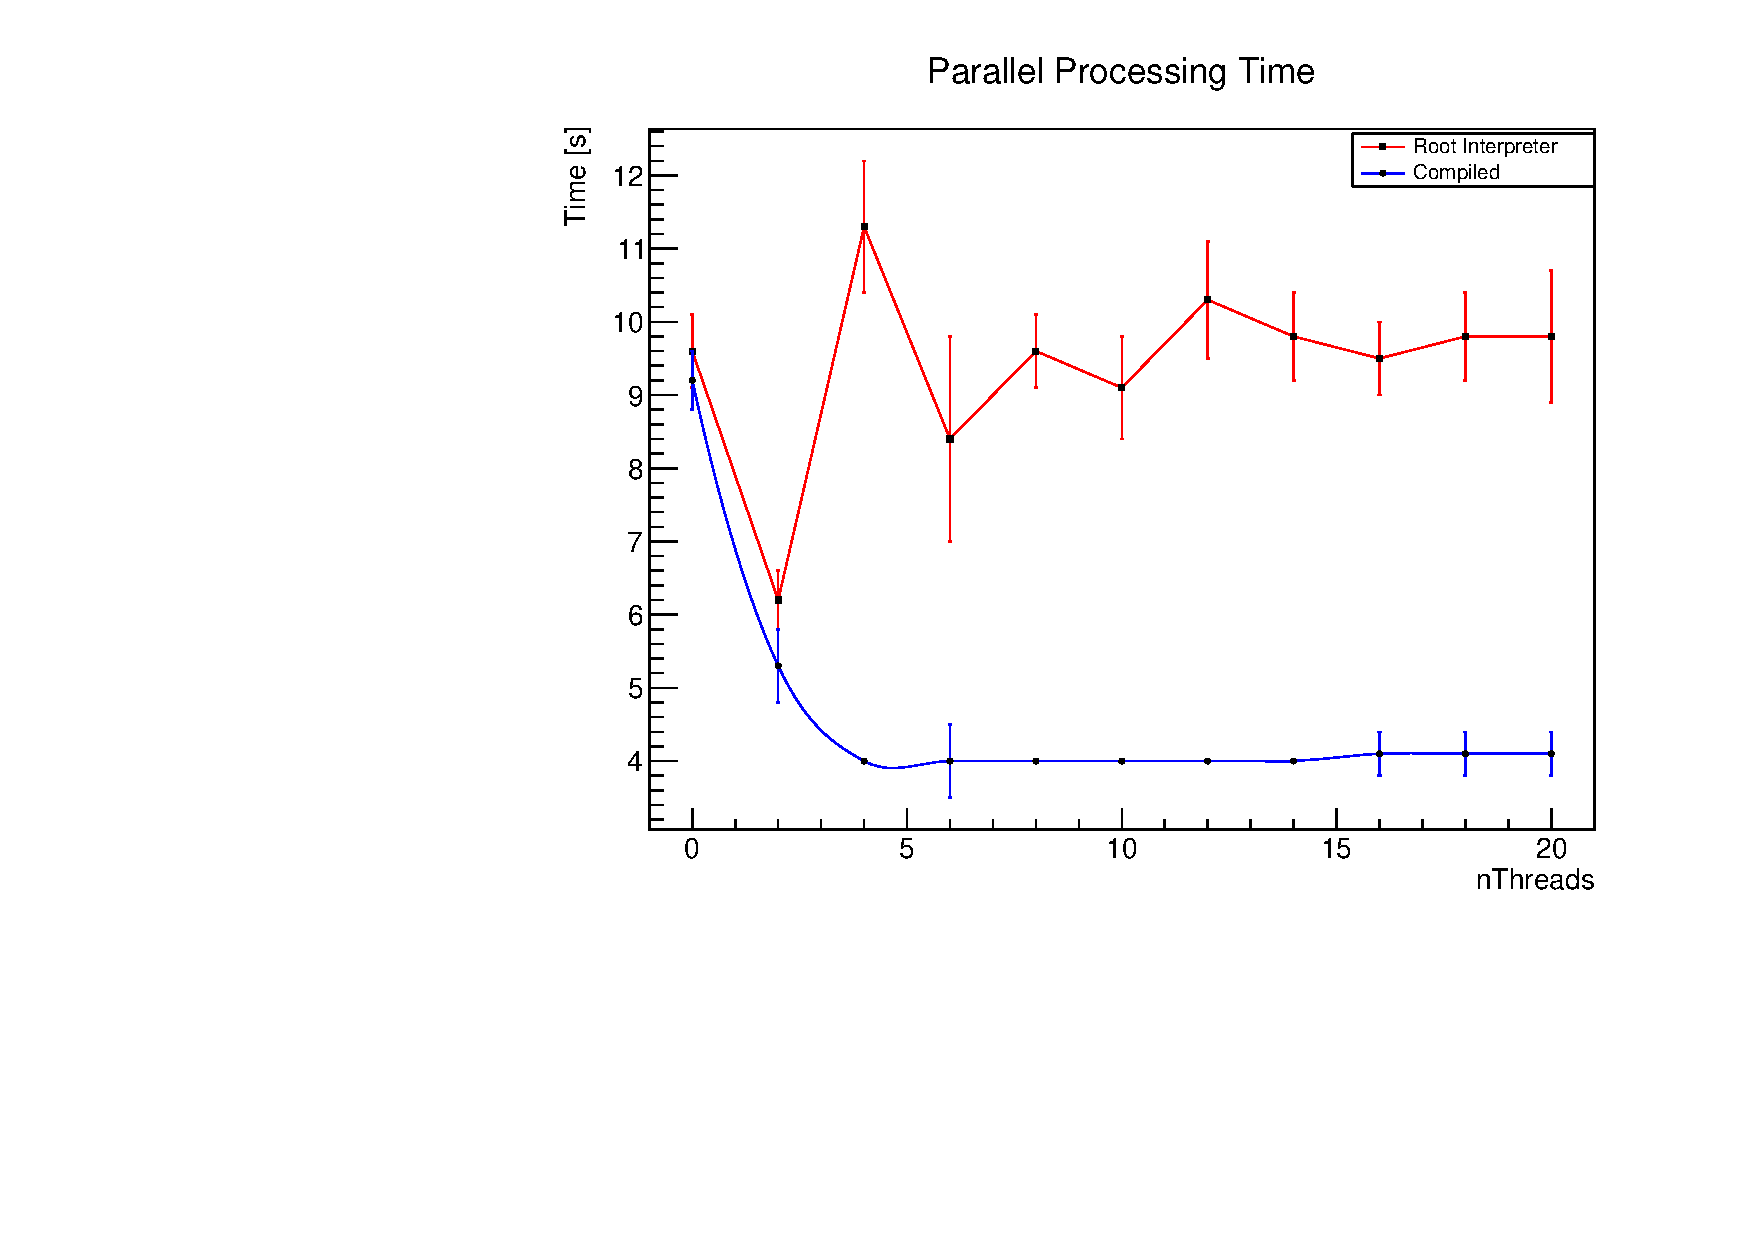
\includegraphics[scale=0.3, left]{../ParTree/test1plot.pdf}

	\end{column}
\end{columns}
\end{frame}

\begin{frame}
Second attempt using ROOT6 parallelization versus classic(Make Class) sequential program (my current approach) on  t3.unl.edu\\
Methods:\\
\begin{itemize}
\item Sequential run over multiple test files with TTreeReader (Compiled Only)
\item Parallelized run over multiple test files with TTreeReader (Compiled Only)
\item Sequential run over multiple test files with MakeClass (Compiled and Interpreted)
\end{itemize} 

Test File set Details:\\
\begin{itemize}
\item using 9 files from Dataset: \url{/SingleMuon/Run2018D-PromptReco-v2/AOD }
\begin{itemize}
\tiny
	\item Physics group: NoGroup Creation time: 2018-08-01 13:16:41 Status: VALID Type: data Dataset size: 150070502441346 (150.1TB) Number of blocks: 267 Number of events: 511823047 Number of files: 45330 
	\end{itemize}
\normalsize
\item 1576737 events each with at least 1 conversion per event
\item total tracks overall (exactly 2 per conversion) = 14190956   
\end{itemize}

\end{frame}

\begin{frame}
File Sequence Details:\\
\begin{columns}
	\begin{column}{0.5\textwidth}
\scriptsize
\begin{itemize}
    \item \url{Run2018_100.root} 
         \begin{itemize}
         	\scriptsize
      		\item   contains 193388 events
       		\item  contains 1547322 unique conversion tracks
        \end{itemize}
   \item \url{Run2018_110.root}
        \begin{itemize}
        \scriptsize
     		 \item   contains 140502 events
     		\item   contains 950444 unique conversion tracks
        \end{itemize}
   \item \url{Run2018_120.root}
        \begin{itemize}
        \scriptsize
      		 \item  contains 99085 events
      		 \item  contains 602330
        \end{itemize}
    \item \url{Run2018_130.root} 
        \begin{itemize}
        \scriptsize
       		\item  contains 62289 events
       		\item  contains 347156 unique conversion tracks
        \end{itemize}
   \item \url{Run2018_141.root}
        \begin{itemize}
        \scriptsize
      		\item  contains 218339 events
       		\item  contains 1958272 unique conversion tracks
        \end{itemize}
        \end{itemize}
        \end{column}
        \begin{column}{0.5\textwidth}
	\scriptsize
		\begin{itemize}
   \item \url{Run2018_155.root}
        \begin{itemize}
        \scriptsize
      		\item   contains 269483 events
      		\item   contains 2968340 unique conversion tracks       
        \end{itemize}
   \item \url{Run2018_166.root}
        \begin{itemize}
        \scriptsize
      		 \item  contains 172409 events
       		\item  contains 1299172 unique conversion tracks
        \end{itemize}

    \item \url{Run2018_176.root}
        \begin{itemize}
        \scriptsize
      		\item   contains 127117 events
      		\item   contains 832024 unique conversion tracks
        \end{itemize}
    \item \url{Run2018_193.root}
        \begin{itemize}
        \scriptsize
      		 \item  contains 294125 events
       		\item  contains 3685896 unique conversion tracks 
        \end{itemize}
\end{itemize}
\end{column}
\end{columns}

\end{frame}

\begin{frame}
First Cluster Test Results:\\
\tiny
(Using full 9 file dataset)\\
\begin{columns}
	\begin{column}{0.5\textwidth}
	\begin{itemize}
		\scriptsize
		\item Time is Mean time $\pm$ stdev over 5 trials
		\item data point at nThreads = 0 is the basic sequential program
		\item high threadcount again not optimal, chokes up the system
		\item Classic sequential approaches using MakeClass (Compiled and Interpreted)--
			\begin{itemize}
				\scriptsize
				\item $265.4 \pm  20.6$ [s] (Interpreted)
				\item $171.0 \pm  23.7$ [s] (Compiled)

			\end{itemize}
		\item ROOT6 mutlithreading is very good!
	\end{itemize}
	\end{column}
	\begin{column}{0.5\textwidth}
   		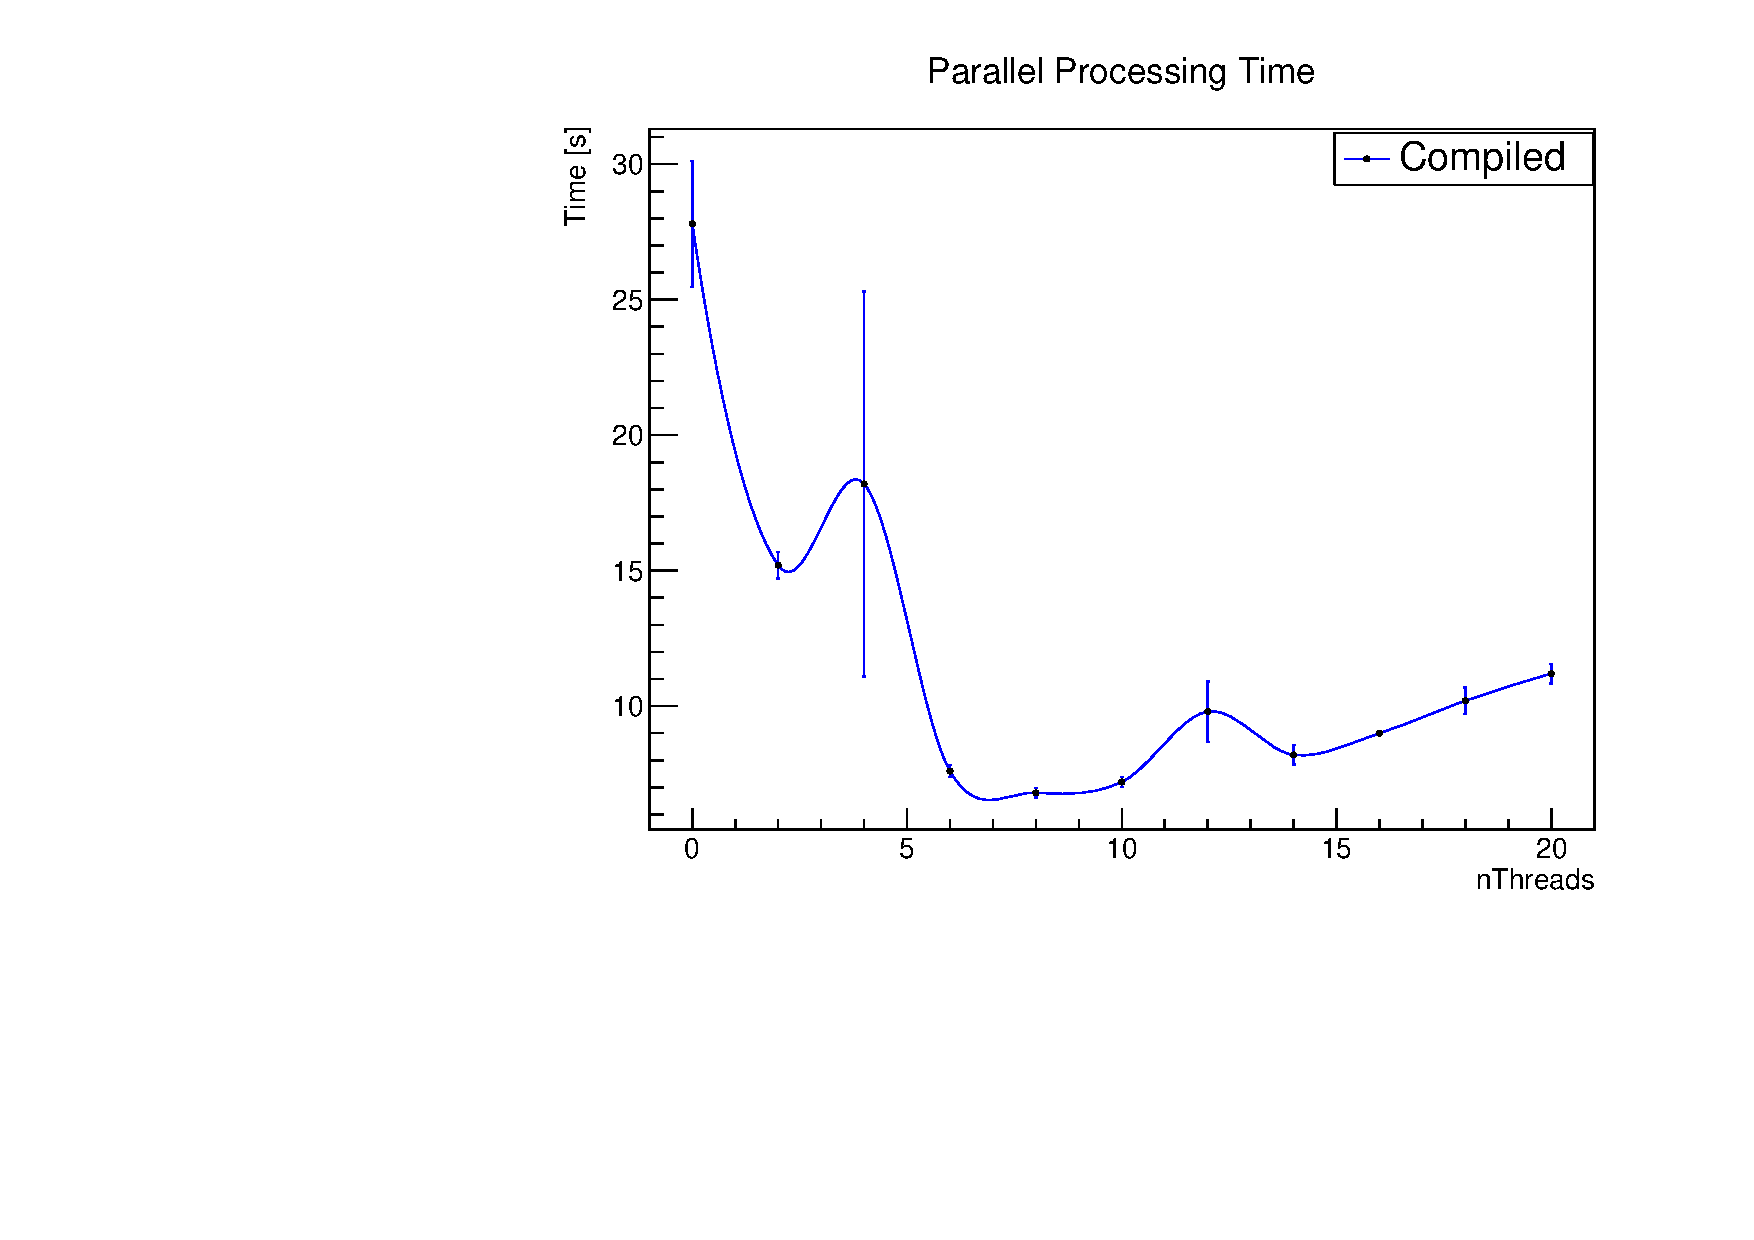
\includegraphics[scale=0.3, left]{../ParTree_t3/test1plott3.pdf}

	\end{column}
\end{columns}

\end{frame}

\begin{frame}
Second Cluster Test:The impact of data size on performance\\
\begin{columns}
	\begin{column}{0.5\textwidth}
		\scriptsize
	\begin{itemize}
		\item Time is Mean time $\pm$ stdev over 5 trials
		\item nTracks is the accumulated number of tracks looped over for a given number of files that are run in a preserved order
		\item Parallel is run with the previously optimal number of threads (8)
		\item Parrellization is faster and more consistent at any size of dataset 
		\item As data gets larger the parallel benefit becomes more significant
	\end{itemize}
	\end{column}
	\begin{column}{0.5\textwidth}
   		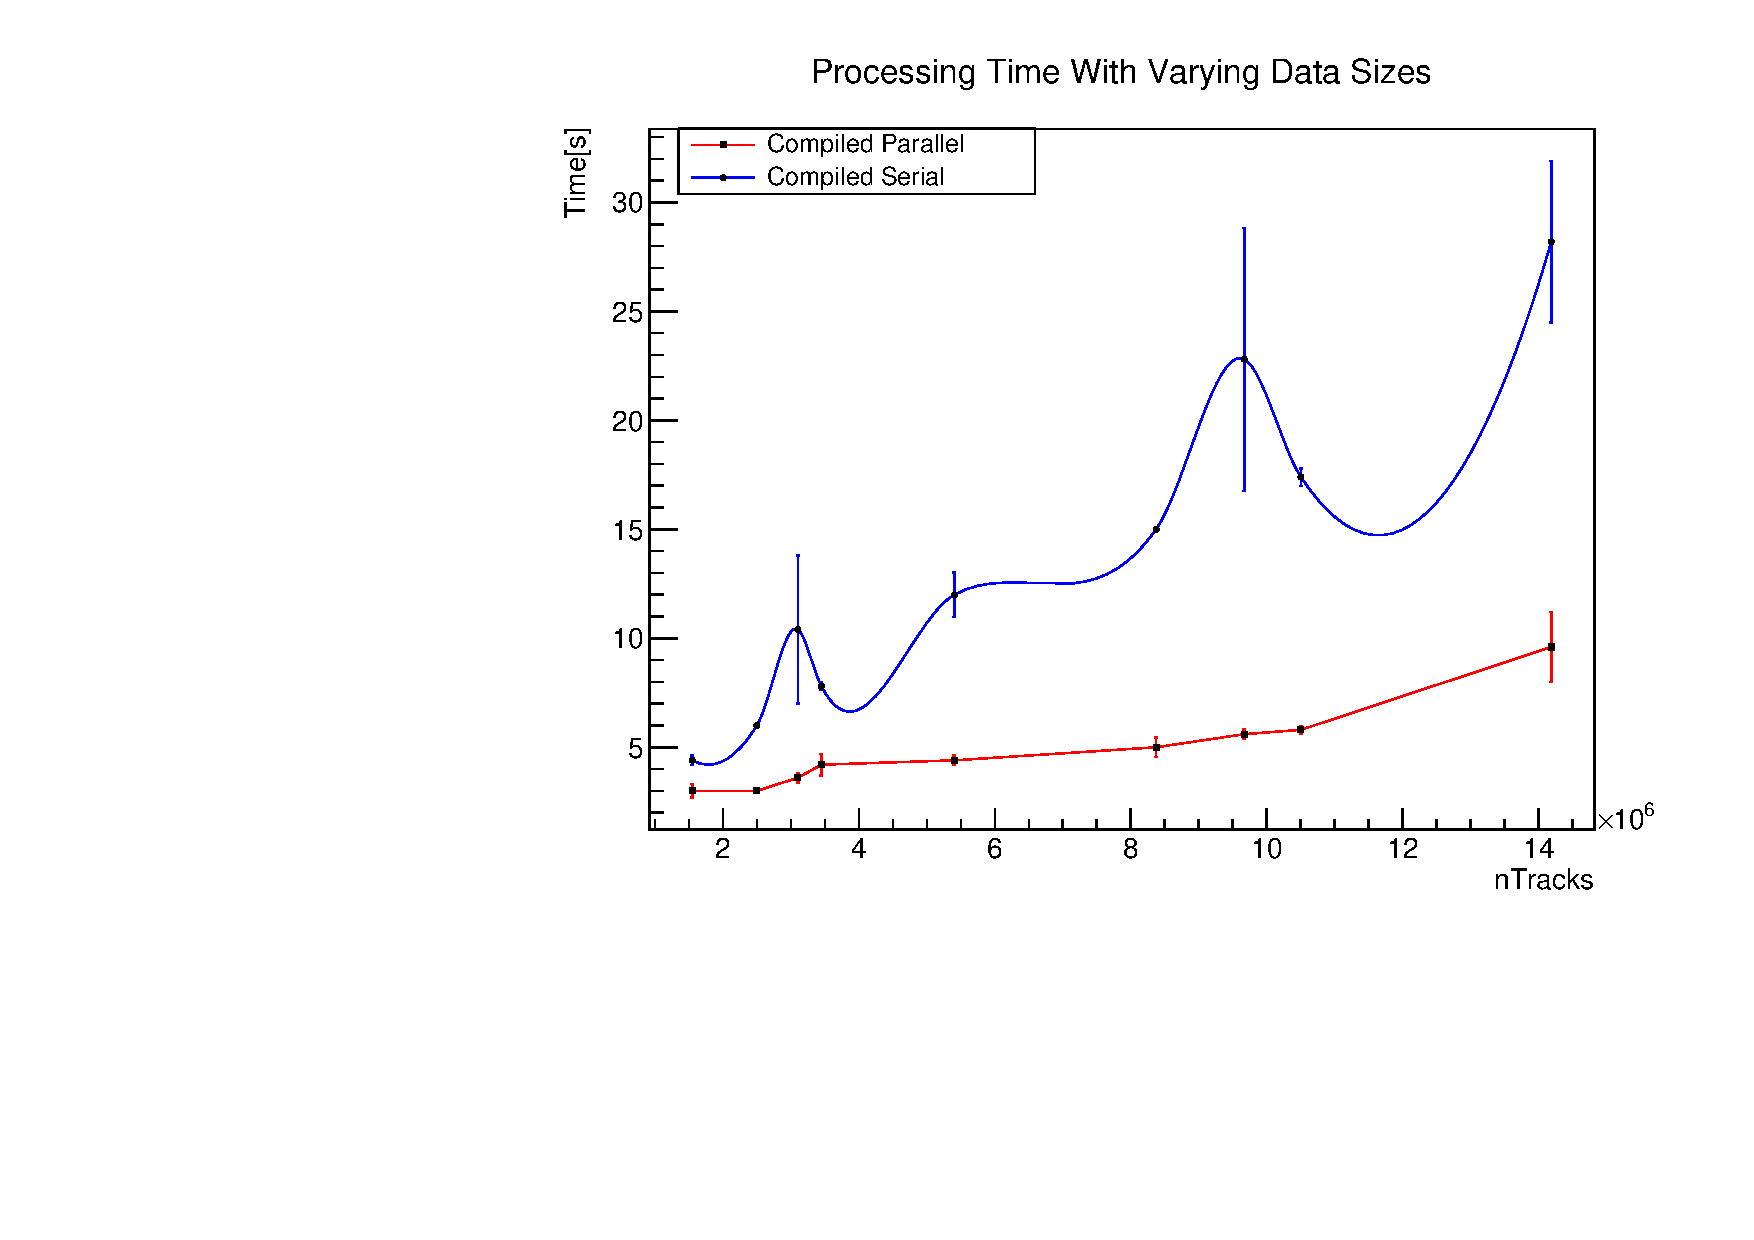
\includegraphics[scale=0.3, left]{../ParTree_t3/sizetestt3.pdf}
	\end{column}
\end{columns}

\end{frame}
\end{document}